\chapter{Protein Location Relation Extraction: Materials \& Methods}\label{chapter:methods}
\newcommand*{\xml}[1]{\texttt{<#1>}}
%\section{Task Definition}

%TODO Refer to the actual section of relatione extraction
This chapter explains the method developed to extract the protein-location relations from the biomedical text. The task of relation extraction is one of the semantic tasks in the area of natural language processing (NLP), as explained in the section \ref{sec:RE}.

The task of protein-location relation extraction can be formally described as follows: given a piece of text that contains two entity mentions, viz. protein and location, decide if the text contains enough evidence for a semantic relationship between these two entities. Formally, let $r=(t,arg_1,arg_2)$ denote a relationship instance where $t$ is a piece of text, $arg_1$ and $arg_2$ are entity mentions contained in text $t$, and $arg_1$ precedes $arg_2$ in the text. Given a set of relations $\left\lbrace r_i \right\rbrace$ such that every relation instance has label $l \in \left\lbrace-1,1\right\rbrace$, our task is to learn a function that can predict the label $l$ for a new relation instance whose label is not known. Note that $t$ can simply be a piece of text or it may also contain structured information such as a parse tree or a dependency graph. For entity mentions $arg_1$ and $arg_2$, either of them can represent a protein or a location entity.

% Following section to be deleted, to be shifted to introduction
\section{Replication of the state of the art in BioNLP'09}

% where should I put that
Section \ref{sec:JariBioNLP} describes the method developed by Björne et al. \cite{bjorne2009extracting} for the task of event extraction in BioNLP 2009. This along with several other methods for various tasks is available online at \url{http://jbjorne.github.io/TEES/}. I used the package TEES (Turku Event Extraction System) \cite{teesonline} to get started and tried to replicate the results for the task of event extraction. The selection of features in our model is influenced by the features used for the task of event extraction in TEES.

%\section{Method for protein-location relation extraction}
\subsection*{Outline of the chapter}

Section \ref{sec:ssModeldsModel} explains the motivation for creating more than one machine learning model. Section \ref{sec:pipeline} outlines the flow of information in the task of relation extraction. Section \ref{sec:graphRep} explains the actual representation of the data in the model. The process of feature extraction and feature selection is explained in Section \ref{sec:featExp} and \ref{sec:featSel} respectively.

The training methodologies are explained in Section \ref{sec:training}. Section \ref{sec:experiments} describes the effect of different experiments on the the method's performance. Section \ref{sec:evaluationCriteria} explains the evaluation criteria used for calculating the models' performance. Finally, Section \ref{sec:tools} describes some external tools used in my implementation.

\section{Multiple ML models: SSModel and DSModel}\label{sec:ssModeldsModel}

A protein-location relation is a semantic relation between a protein entity and a location entity present in the text. As explained in Section \ref{sec:corpusStats}, protein-location relations are categorized into two key categories, viz. same-sentence relations and different-sentence relations. Same-sentence relations are the relations in which both protein and location entity are present in the same sentence. Different-sentence relations are the ones in which either of the participating entities lie in a different sentence.

As discussed in Section \ref{sec:corpusStats}, around 63.81\% of total protein-location relations are same-sentence relations while the remaining 36.19\% are different-sentence relations. A sentence can be considered as a unit of text, which follows strict grammatical rules. The rules that define the relationship between entities in the same sentence can be different from the rules that define the relationship between entities in the different sentence. This also implies that the feature set for extracting same-sentence relations could be different from the one used for extracting different-sentence relations. Combining both feature sets can possibly decrease the performance of both sub-tasks, viz. same-sentence protein-location relation extraction and different-sentence protein-location relation extraction. Therefore, we decided to develop two machine learning models, one for each sub-task.

Furthermore, the semantic relationship between protein and location in the case of different-sentence relations with large sentence distances might be difficult to extract due to incremental noise. Hence, we focused only on those different-sentence relations, which have a sentence distance of 1, i.e., the protein and location entities are found in a neighboring sentence.

The same-sentence model designed for extracting same-sentence relations is referred as \textit{SSModel} hereafter for the purpose of brevity. The different-sentence model is referred as \textit{DSModel}.

\section{Extraction Method pipeline}\label{sec:pipeline}

%- Explain the whole pipeline
%- Corpus-->Sentence Segmentation-->Tokenization-->Syntactic & dependency Parsing-->Graph Representation-->  Feature Extraction --> ML Model training -->Classification on Test
%- Put a nice picture explaining the pipeline

The overall relation extraction method consists of the following major stages:

\begin{enumerate}

\item \textbf{Data collection \& Corpus creation}

LocText corpus's annotations are formatted in JSON files and can be downloaded on the tagtog web interface: \url{https://www.tagtog.net/-corpora/loctext}. However, the JSON files only contains the text of the annotations. The whole document texts are present in a separate set of HTML files. Every JSON or HTML file corresponds to a particular MEDLINE \cite{medline} document.

To avoid re-calculating model features, I decided to create a XML file containing all the corpus data along with annotations and structural details like parse tree, dependency graphs, etc. Figure \ref{fig:corpusCreation} outlines the process  of corpus creation. The data read from a HTML file is parsed using the Stanford CoreNLP pipeline \cite{manning2014stanford}. In every HTML file, the data is divided into title and abstract (for abstracts). The text is first segmented into sentences (\textit{Sentence Splitting}). Every sentence is then split into tokens (\textit{Tokenization}). Predicted part-of-speech tags are assigned to every token (\textit{Syntactic Parsing}). Finally, the dependency relations between the tokens in the sentence are computed (\textit{Dependency Parsing}). The steps of \textit{Tokenization}, \textit{Syntactic Parsing} and \textit{Dependency Parsing} are repeated for every sentence. These stages of processing are explained in detail in Section \ref{sec:NLPPipeline}.

\begin{figure}
\centering
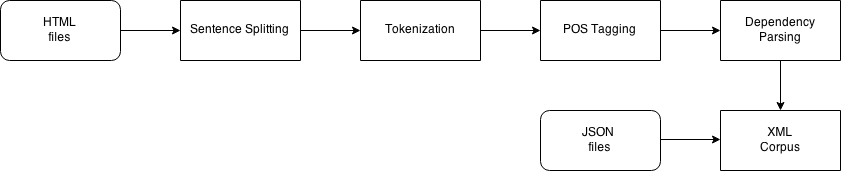
\includegraphics[scale=0.58]{figures/Corpus_Creation.png}
\caption{The process of creating a XML corpus file.}\label{fig:corpusCreation}
\end{figure}

All unstructured (plain text) and structured (sentences, tokens, POS tags, dependencies) information is then combined with annotations present in the JSON files and written to the final XML corpus file.

\begin{figure}
\centering
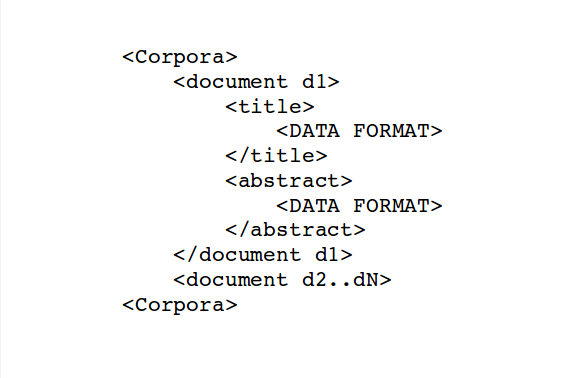
\includegraphics[scale=0.4]{figures/XMLSchema1.png}
\caption{XML file skeleton.}\label{fig:XMLSchema1}
\end{figure}

A coarse skeleton sample of the corpus XML file can be shown in Fig. \ref{fig:XMLSchema1}. Every document (MEDLINE document) has two sections, viz. title and abstract. Both sections have similar structure of internal data representation denoted by \texttt{DATA FORMAT}. The data representation format \texttt{DATA FORMAT} is elaborated in Fig. \ref{fig:XMLSchema2}.

\begin{figure}
\centering
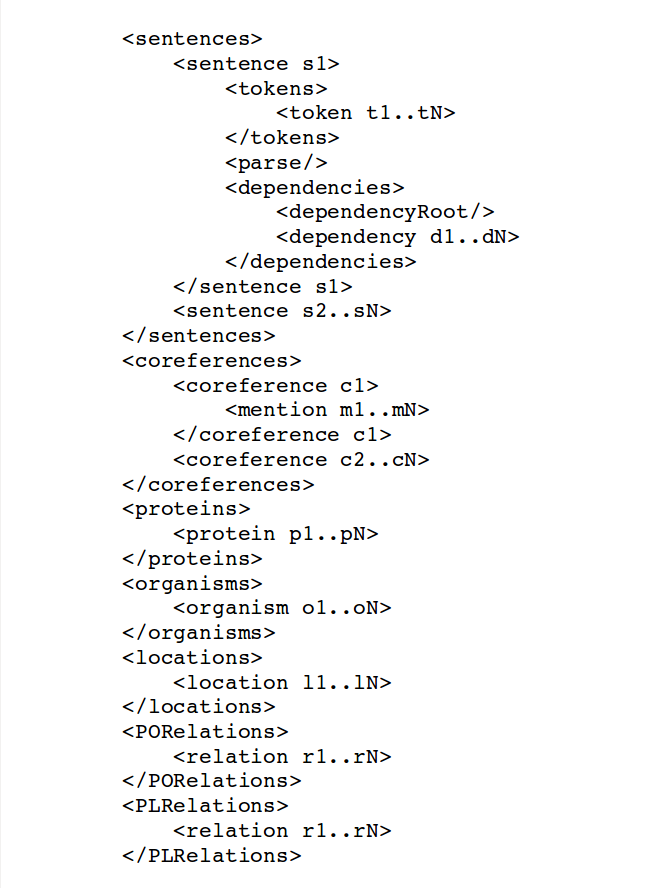
\includegraphics[scale=0.4]{figures/XMLSchema2.png}
\caption{Data format common to title and abstract node}\label{fig:XMLSchema2}
\end{figure}

The \texttt{DATA FORMAT} shown in Fig. \ref{fig:XMLSchema2} represents the XML format used to store the data inside the title and the abstract node. The nested nodes are displayed with a tab indentation. The figure is representative and does not repeat the structures of the nodes for similar parent nodes. For example, even though only the node \texttt{sentence s1} shows the structure of internal nodes like \texttt{tokens}, essentially all the sentence nodes \texttt{sentence s2..sN} have the same structure of the internal nodes.

The nodes in the \texttt{DATA FORMAT} are:

\begin{itemize}
\item \texttt{sentences}: This node represents collection of sentences.
  \begin{itemize}
  \item \texttt{sentence}: a basic sentence unit containing information such as sentence text, start offset, end offset, etc.
    \begin{itemize}
	\item \texttt{tokens}: collection of tokens
	  \begin{itemize}
	  \item \texttt{token}	: a basic token unit containing information such as text of the token, start offset, end offset, POS tag, etc.
	  \end{itemize}
	\item \texttt{parse}: a syntactic parse tree of the sentence
	\item \texttt{dependencies}: collection of dependencies between the tokens
	  \begin{itemize}
	  \item \texttt{dependency}: a dependency relation containing information such as from token, to token, dependency type, etc.
	  \end{itemize}
	\end{itemize}
  \end{itemize}
  \item \texttt{coreferences}:
    This node is a collection of coreferences present in the entire text unit (title or abstract)
    \begin{itemize}
    \item \texttt{coreference}: a collection of coreferent mentions
    \begin{itemize}
      \item \texttt{mention}: This node contains information about the text of the coreferent mention, start token in the sentence, end token and whether this is a representative mention or not.
    \end{itemize}
    \end{itemize}

\item \texttt{proteins}: protein entity annotations
\item \texttt{organisms}: organism entity annotations
\item \texttt{locations}: subcellular location entity annotations
\item \texttt{PORelations}: protein-organism relation annotations
\item \texttt{PLRelations}: protein-location relation annotations
\end{itemize}

\item \textbf{Training \& evaluating \textit{SSModel}}

This is the third stage in the relation extraction method. This stage focuses solely on extracting same-sentence protein-location relations from text.

The data is read from the corpus XML file and stored in internal data structures in the main memory. Reading the file once also saves unnecessary I/O accesses and improves the execution time by a small margin.

Since this step tries to extract the protein-location relations present in a same sentence only, every sentence in the document is analyzed one by one. In every sentence, potential protein-location relations are found out and the features are written for each one of them along with the target label. A relation is considered a potential relation if both the protein entity and the location entity are present in the same sentence. The potential relations that are actually present in the manual annotations are considered true relations and are denoted by target label $1$. On the other hand, the potential relations that are not found in the manual annotations are considered negative relations and are denoted by target label $-1$. Every relation is written as a feature vector. The support vector machine library $SVM^{light}$ \cite{joachims1999making} is used for the purpose of training and classification.  The data representation for $SVM^{light}$ is discussed in more detail in Section \ref{sec:training}.

The data is broken down into training set, development set and test set. A feature file is created each for training set, development set and test set. These files are then used by $SVM^{light}$ to train the classifiers. A model is learned from the training data. This model classifies the examples in the development set and test set. The development set is used for the tuning of the hyperparameters. The model classifies the test set examples using hyperparameter learned on the development set. The process of training and cross-validation is explained in detail in Section \ref{sec:training}.

The results of the classification are then evaluated. Various evaluation criteria used for the evaluation of results are discussed in Section \ref{sec:evaluationCriteria}. The results of the \textit{SSModel} are also cached for use during \textit{DSModel} evaluation later.

\item \textbf{Training \& evaluating \textit{DSModel}}

This third stage aims to extract different-sentence relations. As discussed in Section \ref{sec:ssModeldsModel}, a model is trained for extracting different-sentence relations with sentence distance of 1. A different-sentence relation with sentence distance of 1 implies that the participating protein and location entities are in the neighboring sentence. As done during the training and evaluation of \textit{SSModel}, the data is read from the corpus XML file once and stored in the internal data structures.

For every document, the sentences are processed in pairs and every pair consists of neighboring sentences. The potential different sentence protein-location relations are found out and the relations are written to the SVM feature file. A potential protein-location relation is the one which has participating entities in neighboring sentences. For example, if sentences \texttt{s1} and \texttt{s2} are being processed, then the protein entities in \texttt{s1} can have a potential PL relationship with location entities in \texttt{s2} and vice versa.

Features are extracted for all potential relations and are written to the feature file along with the target label. As done during the training and evaluation of \texttt{SSModel}, a feature file is created each for the training set, development set and test set.

The results of the classification are evaluated using various evaluation criteria discussed in Section \ref{sec:evaluationCriteria}.

\item \textbf{Combined evaluation}

This is the fourth and last stage in the pipeline of relation extraction method. This stage primarily combines the predictions of \texttt{SSModel} and \texttt{DSModel}. The combined predictions are compared with original target labels and evaluated. Unique and non-unique evaluation modes are explained in Section \ref{subsec:UniqNonUniqEval}.

\end{enumerate}

\section{Graph representation} \label{sec:graphRep}
% Details about graph representation along with nice explanatory picture

For the purpose of feature extraction, the data is also used in the form of a graph. Specifically, sentences are represented as a graph, their tokens are the nodes of the graph and the dependency relations between the tokens are the edges in the graph. The models \textit{SSModel} and \textit{DSModel} use different a graph representation, which is explained in the following subsections.

\subsection{Graph representation for \textit{SSModel}}\label{sec:graphSSModel}

%TODO change figure
\begin{figure}
\centering
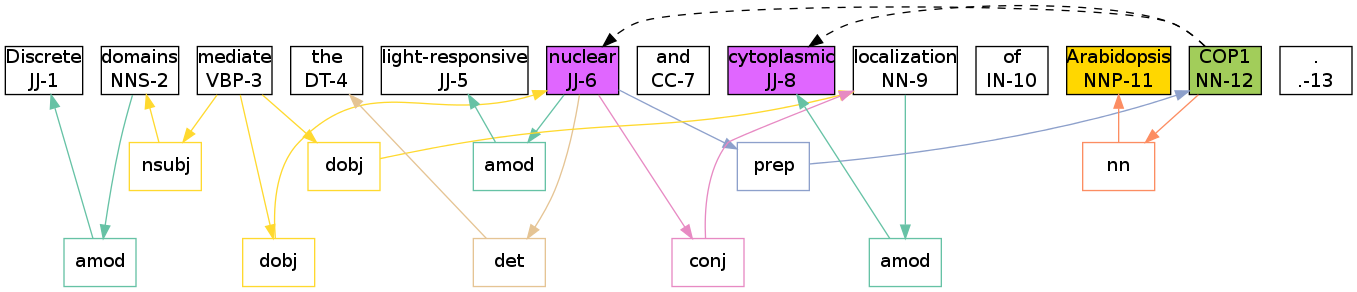
\includegraphics[scale=0.3]{figures/SameSentenceGraph.png}
\caption{Graph representation of a sentence in \textit{SSModel}}\label{fig:SSGraph}
\end{figure}

The representation of a sentence as a graph is shown in Fig. \ref{fig:SSGraph}. The sentence \textit{"Discrete domains mediate the light-responsive nuclear and cytoplasmic localization of Arabidopsis COP1."} is tokenized and every token forms a node in the graph. A displayed node shows the text of its token in the first row and its part-of-speech (POS) tag and the token number joined by a hyphen in the second row. Tokens that are part of a protein entity are shown with a green background, tokens that are part of a location entity are shown with a magenta background and tokens that are part of organism entity are shown with a yellow background. As seen in the graph, \textit{"COP1"} is a protein entity, \textit{"Arabidopsis"} is an organism name and \textit{"nuclear"} and \textit{"cytoplasmic"} are the locations mentioned in the sentence. The nodes in the graph are connected by edges, which are the dependency
 relations between the tokens. The type of the edges are shown with colored boxes. For example, there is a dependency edge of the type \textit{amod} from the token \textit{"domains"}  to  the token \textit{"Discrete"}. Since the dependency relations between the tokens are directed, this graph representation is a directed graph.

Also shown are dashed edges, which represent the protein-location relations. Obviously, these dashed edges are just shown for representation and do not form edges in the actual model graph.

\subsection{Graph representation for \textit{DSModel}}\label{sec:graphDSModel}

%TODO add figure for multi sentences

For \textit{DSModel}, the graph representation is a bit different compared to that in \textit{SSModel}. In \textit{DSModel}, pair of sentences are considered where every pair consists of the two neighboring sentences. Figure \ref{fig:DSGraph} shows an example of \textit{DSModel} graph representation. Similar to the graph representation in \textit{SSModel}, the sentence is tokenized and every token forms a node in the graph. The tokens that are part of protein entity are in green, those part of organism entity are in yellow and the tokens that are part of a location entity are in magenta. Since two sentences are considered at a time, the graphs of these sentences are concatenated together and considered as a combined sentence as shown in Fig. \ref{fig:DSGraph}.

\begin{figure}
\centering
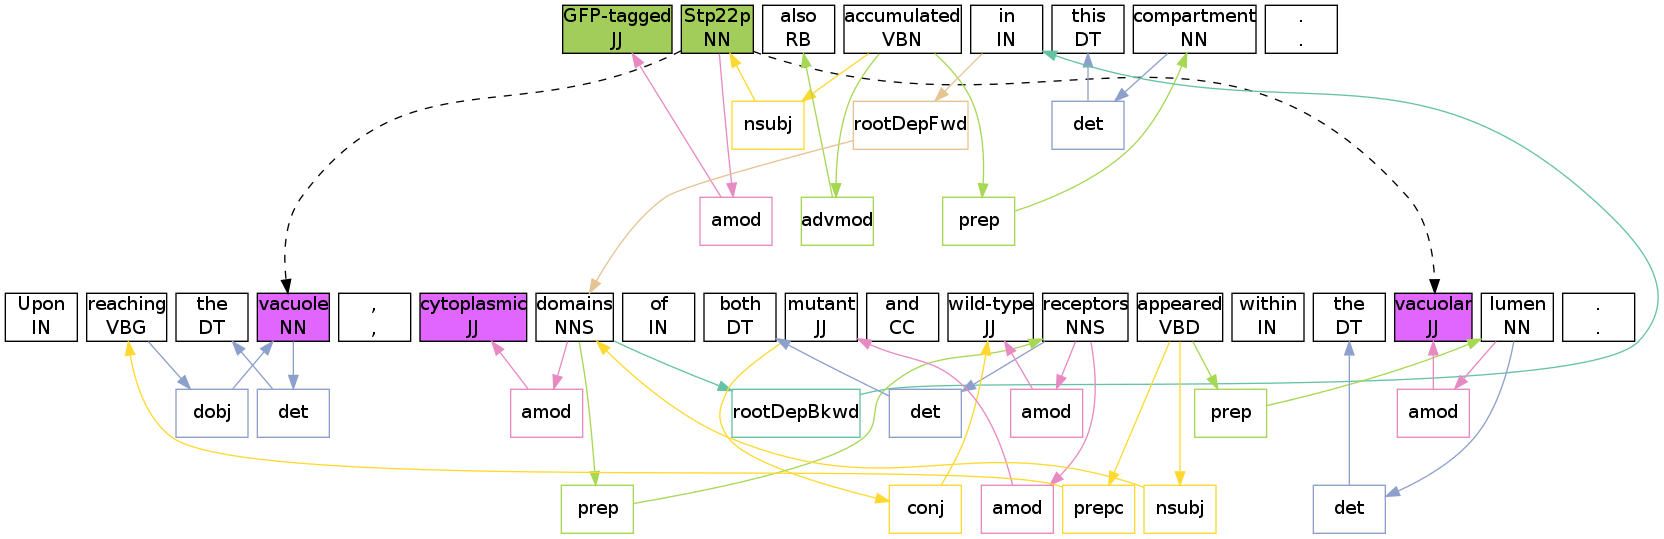
\includegraphics[scale=0.3]{figures/DiffSentenceGraph.png}
\caption{Graph representation of a combined sentence in \textit{DSModel}}\label{fig:DSGraph}
\end{figure}

The edges in the graph are primarily dependency edges between the tokens in two sentences. In addition to the dependency edges, the graph is augmented with several other edges. The additional edges are:

\begin{itemize}

\item \textbf{Root to root connection}: the root of the first sentence is connected with the root of the second sentence. This connection helps in finding the path from a entity in one sentence to an entity in another sentence. This connection is bidirectional. As shown in Fig. \ref{fig:DSGraph}, the root of the first sentence \textit{"in"} is connected via a dependency edge to the root of the second sentence \textit{"domains"}. The forward dependency edge between the roots is labeled \textit{rootDepFwd} and the backward dependency edge between the roots is labeled \textit{rootDepBkwd}.

\item \textbf{Connections between same words}: if some of the tokens in both sentences are nouns and have similar text, then these tokens are connected by edges. These edges are directed from tokens in the first sentence to the tokens in the second sentence.

\item \textbf{Connections between protein entity and "protein" word}: these are special connections that try to gauge coreferent mentions in the most naive manner. If one of the sentence contains a word "protein" and does not contain any protein entity, then it is likely that the word "protein" in this sentence may actually be referring to the protein entities in other sentence. Therefore, a connection is made from the word "protein" to the protein entities in other sentence with the expectation that if this is a case of coreferent mention, then it will be easier to extract the path.

\item \textbf{Connections between location entity and "location" word}: with the similar assumption as mentioned in the previous point, it is assumed that if a sentence has a word "localize", "location" or "compartment" and it does not have a location entity, then it might be the case that this word is a coreferent mention of the location entity present in the other sentence. Therefore, an extra edge is added between the words containing text "location", "localize" or "compartment" to the location entity. This is a directional edge from the word to the entity. In Fig. \ref{fig:DSGraph}, although there is a word \textit{compartment} in the first sentence, the connection are not shown to keep the figure readable.

\end{itemize}

For instance, in Figure \ref{fig:DSGraph}, the entity \textit{Stp22p} of the first sentence has a PL relationship with location entities \textit{vacuole} and \textit{vacuolar} present in the second sentence. These edges are denoted by dashed lines. As mentioned previously, the dashed edges are just for the purpose of illustration and do not form true edges in the graph used for feature extraction. In this way, \textit{DSModel} considers the combination of two neighboring sentences as a single sentence unit and extracts the features from such a combined sentence.

%\section{Data Structures} \label{sec:dataStructure}

\section{Feature extraction}\label{sec:featExp}

This section explains the process of feature extraction. The format of the feature set to be written for $SVM^{light}$ is explained in detail in Section \ref{sec:training}. Although there are a few differences in the feature sets of \textit{SSModel} and \textit{DSModel}, most of the features are common to both models.

There are three sources from which the features can be extracted, namely: sequences (text), syntactic parse trees and dependency parse trees \cite{jiang2007systematic}. A variety of features are extracted from all these sources and combined for optimal performance. An overview of the features can be presented as follows.

\subsection*{Sentence features}

Sentence features are extracted for every potential relation that is a part of the sentence. Sentence features include bag of words (BOW) of tokens in the sentence, stem of tokens in the sentence and frequency features like number of protein entities in the sentence, number of location entities in the sentence, number of organism entities in the sentence, count of the bag of words, etc.

\subsection*{Token features}

Token features are extracted for tokens that are part of the entities and for tokens that are in a linear dependency with the entities. Every entity is represented by a head token, which is calculated by a simple heuristic. % j: which heuristic?

% j: what is masked token text?
Token features include token text, masked token text, stem, POS tag, etc. Most of the features are binary and some are integer-valued features. There are features for binary tests on a token, e.g., whether the first letter of token is in capital case or not (capitalization test), whether some letter in the middle is in capital case or not, etc.. Other binary tests include presence of a hyphen, presence of forward slash, presence of backward slash, presence of digits, etc.. Character bigrams and trigrams of the token also contribute to the token features.

\subsection*{Linear context and dependency chain}

Token features are also extracted for tokens that are present in the linear and dependency context. A linear context of length 3 is considered, i.e., features are extracted for the next and previous 3 tokens relative to the token under consideration.

A dependency chain of length 3 is considered for the dependency context. Incoming and outgoing dependencies are considered for dependency-related features. For example, in the case of incoming dependencies, features are extracted for the \emph{source}/\emph{from} token and its incoming and outgoing dependencies are considered too. This goes on up to a dependency depth of 3. In addition to the token features, the dependency edge types are also considered while extracting dependency chain features.

\subsection*{Dependency features}

\begin{figure}
\centering
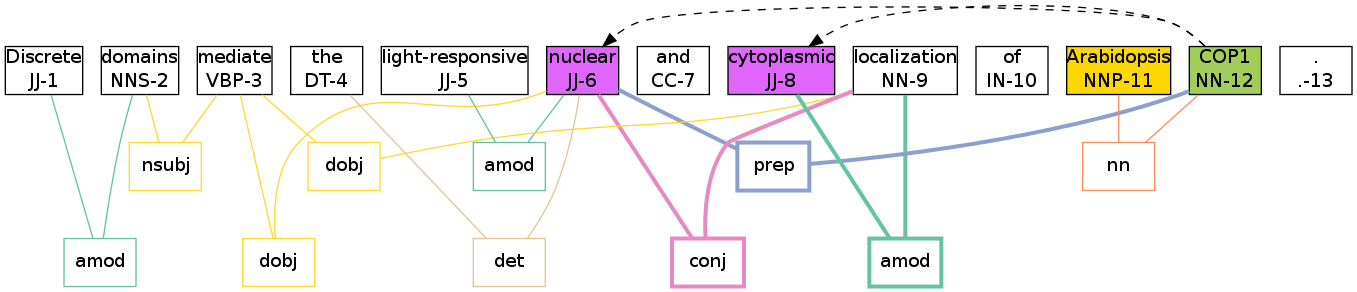
\includegraphics[scale=0.3]{figures/ShortestPath.png}
\caption{Shortest Path from protein entity \textit{COP1} to location entity \textit{cytoplasmic}}\label{fig:shortPath}
\end{figure}

Many features are extracted depending on the dependency graph. Using the Floyd-Warshall algorithm, the shortest path between a protein entity and a location entity in a potential PL relation is calculated. For the purpose of extracting the shortest path, an undirected graph of dependencies is considered. Figure \ref{fig:shortPath} shows the shortest path from protein entity \textit{"COP1"} to location entity \textit{"cytoplasmic"}. The path is shown in bold. Note that an undirected graph is considered only for the purpose of extracting the shortest path. Most of the dependency-based features depend on this shortest path. While extracting the features, the original direction of the edges in the shortest path is also taken into consideration. The length of the shortest path contributes an integer-valued feature in addition to the binary feature for each length.

Token features are extracted for terminal features of the shortest path, which are head tokens of the entities. Some of the other path related features include token features of the internal tokens in the path, features for every edge in the path, features for internal edges in the path, etc.

\subsubsection*{N-gram dependency features}

The protein and location entities are represented by their respective head tokens. The shortest path between two entities is actually a shortest path between the head tokens. However, there need not be a single shortest path between two entities. There can be multiple paths between two entities with same distance or same minimum distances. All such paths with minimum distance are computed and features are extracted for each one of them.

For every such minimum distance path from the set of minimum distance paths, parts of the paths are considered for N-gram features. For example, a set of all 2 consecutive tokens are considered for 2-gram features and a set of all 3 consecutive tokens are considered for 3-gram features, etc.. 2-, 3- and 4-gram features are extracted from all such paths. These features also include token features that are part of the corresponding set, dependencies in the set, directions of dependencies in the set, etc.

\subsection*{Other features}

Other features include relative order of the entities, the features of the tokens that lie between entities in a potential relation, features depending on the presence of word "protein", presence of other special words between two entities, etc. % j: which 'special' words? List them, if not here, in a footnote or appendix

\subsection*{Features specific to \textit{DSModel}}

Some features are specific to the \textit{DSModel} since it involves processing a pair of sentences as a combined sentence along with extra links. Some of those features include bag of words/stem/POS of tokens in individual sentences, binary tests like the presence of an entity in the first sentence or second sentence, etc. Importantly, the \textit{DSModel} also uses the predictions of the \textit{SSModel}. The features depending on \textit{SSModel} predictions include binary tests like whether the entities considered in the potential relations have a predicted same-sentence relation or not. The intuition behind using same-sentence predictions is that entities that already have a same-sentence relation are unlikely to have a different-sentence relation in most cases.

\section{Feature Selection}\label{sec:featSel}

Feature selection is the process of filtering appropriate features from a large set of possible available features. There are several motivations for feature selection, one of which is to avoid overfitting and improve generalization accuracy. Therefore, the task of feature selection can also be viewed as the task of removing irrelevant features.

%Write some of the results found out from in Joachim's paper [Text categorization with SVM]
%
%**This is a very important property that has got to be known that in text categorization using SVM, there are only few irrelevant features.
%
%When ranked according to Binary information gain, see Figure 1, removal of high ranking features does not take away a lot of information. This also means that even features ranked lowest still contain considerable information and are somewhat relevant.
%

As observed by authors in \cite{joachims1998text}, for the task of text categorization, there are very few irrelevant features. The authors calculated binary information gain for all the features and found out that even the features that are ranked lowest contain considerable information and are somewhat relevant. In the task of text categorization, the documents are classified into one of the several predefined categories depending on the words present in that document. Therefore, the words/terms present in the document are the features for the task of text categorization and it is easier to discard the words/terms if that particular feature is found irrelevant.

However, for our task of relation extraction, the features are very complex and discarding individual features is not an option. The features are extracted with the purpose of extracting some characteristic (e.g. binary test of capitalization in the case of token features) and the entire feature-generating mechanism (e.g. feature-generating function in our case) should be commented out if those features are found ineffective.

Several approaches for the task of feature selection are used and they are explained below.

\subsection{Leave one out}\label{subsec:LeaveOneOut}

For the task of protein-location relation extraction, the feature generators are the functions that extract certain characteristics. Such feature generators are commented out in a \emph{leave-one-out} fashion such that \emph{all} the features extracted by that function are discarded. The performance of the method is then calculated. This process is repeated for all feature generators to find out which feature generators produce irrelevant features. The feature generators, which upon commenting out boost the performance of the model, can be then removed from the final set of feature generators.

This approach results in some performance improvement but the biggest drawback of this approach is the independence assumption. This approach assumes that the features $\left\lbrace {fg_1}_i \right\rbrace$ generated by a feature generator $fg_1$ is independent of the features $\left\lbrace {fg_2}_i \right\rbrace$ generated by feature generator $fg_2$. However, the features in set $\left\lbrace {fg_1}_i \right\rbrace$ and $\left\lbrace {fg_2}_i \right\rbrace$ might not be strictly independent. It may happen that commenting either $\left\lbrace {fg_1}_i \right\rbrace$ or $\left\lbrace {fg_2}_i \right\rbrace$ may not improve any performance but commenting both can. The leave-one-out feature generator approach does not care about combining the feature sets of individual feature generators and therefore, it does not result in the optimal selection of the feature subset.

\subsection{Information gain}\label{subsec:IG}

A widely used technique for feature selection is to calculate the information gain of the features \cite{yang1997comparative}. The information gain is used to calculate the goodness/fitness of the features. The features with higher goodness are kept and others can be discarded. The information gain for the feature $f$ can be calculated as:

\begin{align}
\begin{aligned}
 G \left( f \right) = & -  \sum^m_{i=1} P_r(c_i) \text{ log } P_r(c_i) \\
  & + P_r(f) \sum^m_{i=1} P_r(c_i|f) \text{ log } P_r(c_i|f)\\
  & +  P_r(\overline{f}) \sum^m_{i=1} P_r(c_i|\overline{f}) \text{ log } P_r(c_i|\overline{f})
\end{aligned}
\end{align}

where $c_i$ is the set of target label relations, $\left\lbrace +1, -1 \right\rbrace$, $f$ indicates the presence of the feature and $\overline{f}$ indicates the absence of it.

\subsection{Feature weights}\label{subsec:FWR}

Another relevant approach used for feature selection is normal-based feature selection \cite{brank2002feature}. As discussed in Section \ref{sec:SVM}, support vector machines use a hyperplane to separate the positive instances from the negative ones. For a linear kernel, the prediction for a certain example $x$ can be written as:

$$
prediction(x) = sgn \left[ \mathbf{w}^T\mathbf{x} + b \right]
$$

where $\mathbf{w}$ is the vector of weights. Geometrically, $\mathbf{w}$ is the normal to the hyperplane that is used by the predictor. Authors in \cite{brank2002feature} show that the weights of individual features influence the hyperplane and margin. Therefore, the most significant features are the ones which have highest feature weights. This approach can be used to extract highest-weighted features and discard others.

\section{Training, Cross validation and Classification}\label{sec:training}

All following experiments are performed on the LocText \cite{loctext} corpus (explained in Section \ref{sec:LocTextCorpus}).

\subsection{Representation of examples in $SVM^{light}$ }

$SVM^{light}$ \cite{joachims1999making} has a specific way of representing the instances. For protein-location relation extraction, every potential relation is an instance. Every instance is written on a new line in a plain file and represented as a vector of features. Following format explains the structure of every instance:

\bigskip

\texttt{<line> .=. <target> <feature>:<value>...<feature>:<value> \# <info>}

\texttt{<target> .=. +1 | -1 | 0 | <float>}

\texttt{<feature> .=. <integer> | "qid"}

\texttt{<value> .=. <float>}

\texttt{<info> .=. <string>}

\subsection{Cross validation}

\begin{figure}
\centering
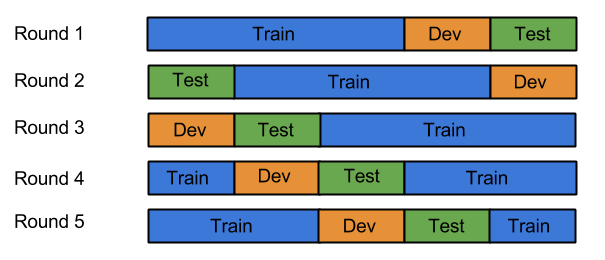
\includegraphics[scale=0.6]{figures/CrossValidation.png}
\caption{5-fold cross validation}\label{fig:crossVal}
\end{figure}

A 5-fold cross validation is used where every fold consists of 20 documents (out of the 100 abstracts). In every round, 60\% of the total data is used for training, 20\% for development and 20\% for test. Since our corpus has 100 documents, 60 documents are used for training, 20 for development and 20 for testing in every round of cross validation. The training data is used to train the model using $SVM^{light}$. The development data is used for tuning the hyperparameters. For both \textit{SSModel} and \textit{DSModel}, regularization parameter $\mathbf{C}$ is the only hyperparameter to be tuned. Finally, unseen test data is used for calculating round performance results. The final performance of the model is the average of the performance for all 5 rounds. Figure \ref{fig:crossVal} illustrates the division of data for 5 rounds of cross validation.

%TODO Add more details about other experimentation
\section{Additional experimentation}\label{sec:experiments}

Several experiments were designed and their effect was observed on the performance of the models. All of these experiments were somewhat based on intuition. This section describes the effects of all such experiments. This section initially describes the experimentation common to \textit{SSModel} and \textit{DSModel}. The experiments specific to \textit{SSModel} and \textit{DSModel} are discussed later as a subsection.

\subsubsection*{Experimentation with different kernels}

$SVM_{light}$ provides an ability to use different kernels for the purpose of training a model. The default kernel is the linear kernel and other kernels are polynomial, RBF (Radial Basis Function) and sigmoid kernels. After experimentation, using kernels other than the default kernel reduces the performance of the method. Even \cite{joachims1998text} shows that the linear kernel is the best kernel that can be used for text processing.

\subsubsection*{Minimum subtree}

\subsubsection*{Path enclosed subtree}

\subsubsection*{Use of coreferences} \label{subsubsec:coref}

\subsection{Experimentation specific to \textit{SSModel}}
%TODO

\subsection{Experimentation specific to \textit{DSModel}}

\subsubsection*{Using additional information}

Efforts were made to increase the performance of \textit{DSModel} using additional information extracted from the document. One instance of such additional information is \emph{shortform}-\emph{longform} pairs extracted from the document. The intuition was that if either the short or long name form of a protein is predicted to be in a protein-location relationship with a particular location entity, then the corresponding short or long form should also be in a protein-location relationship with that entity. \emph{Shortform} and \emph{longform} pairs were extracted using a simple algorithm \cite{hearst2003simple}. However, adding such information actually decreased the performance of \textit{DSModel} since more number of false positives were added than true positives. It was decided, therefore, not to use this augmentation of information.

\section{Evaluation Metrics} \label{sec:evaluationCriteria}

\subsection{Performance measures}

% Precision, Recall, Fscore
The standard performance measures \textit{Precision}, \textit{Recall} and \textit{F score} are used for calculating the performance of \textit{SSModel} and \textit{DSModel}.

For the task of protein-location relation extraction, a positive prediction is the one in which the machine learning model predicts a PL (protein-location) relation between a protein entity and a location entity. Similarly, a negative prediction is the one in which the machine learning model predicts that there is no relation between a protein entity and a location entity.

A prediction can be classified into one of the following categories:


\begin{itemize}

\item \textit{True positive (tp)}: A prediction is said to be a true positive if it is a positive prediction (i.e., the entities are predicted to be related) and it matches an original relation in the corpus.

\item \textit{True negative (tn)}: A prediction is said to be a true negative if it is a negative prediction and the entities in the relation are also not related in the original corpus.

\item \textit{False positive (fp)}: A prediction is said to be a false positive if it is a positive prediction but the participating entities are not related in the original corpus.

\item \textit{False negative (fn)}: A prediction is said to be a false negative if it is a negative prediction even though the participating entities are related in the original corpus.

\end{itemize}

\subsubsection*{\textit{Precision}}\label{subsubsec:Prec}

Precision is the fraction of true predictions from all predictions and is given by:

$$
\textit{Precision} = \frac{tp}{tp+fp}
$$


\subsubsection*{\textit{Recall}}\label{subsubsec:Recal}

Recall is the fraction of original relations that are predicted and is given by:

$$
\textit{Recall} = \frac{tp}{tp+fn}
$$

\subsubsection*{\textit{F score}}\label{subsubsec:Fscore}

F score, also called as F1 score, is the harmonic mean of precision and recall. It is given by:

$$
\textit{F score} = 2 * \frac{Precision * Recall}{Precision + Recall}
$$


%TODO write about standard error

\subsection{Evaluation modes} \label{subsec:Eval}

% Talk about unique relations here
\subsubsection{Unique}\label{subsubsec:UniqEval}

In the unique evaluation mode, a set of unique protein-location relations is made for every document in the corpus, notwithstanding the repetition of relations in the document. A predicted positive relation is said to match with the original unique relation if and only if the predicted relation for the document is found in the set of unique relations for that document. If the predicted relation is not found in the set, it is either classified as a false positive if it is a positive prediction or a true negative if it is a negative prediction.


\subsubsection{Not unique}\label{subsubsec:NonUniqEval}

Simply put, the results of non-unique evaluation mode are the results of SVM classification. The predictions are compared with original relations and the results are computed.

For a particular document in the corpus, it may happen that a protein is related to a location twice or more in the document at different places. In this evaluation mode,  such repetitions are considered separately and therefore, this evaluation mode is called non-unique evaluation mode. For this mode of evaluation, a predicted relation is said to match with an original relation if and only if the text offsets of both protein and location entities in the predicted relation matches exactly with the text offsets of protein and location entities in the original relation respectively.

It is important to note that, in this evaluation mode, SSModel considers the list of same-sentence relations for evaluation, whereas DSModel uses the list of 1-sentence-apart relations. This is in contrast to the unique mode, where the set of all the document's relations are considered to evaluate both SSModel and DSModel.

\section{Tools used}\label{sec:tools}

The Stanford corenlp pipeline \cite{manning2014stanford} is used for sentence segmentation, tokenization, syntactic parsing, dependency parsing and coreference resolution. The support vector machine library $SVM^{light}$ \cite{joachims1999making} is used for training and classification.
